\section{Parallel Series Converter} \label{subsec:PSC}
The Parallel Series Converter or PSC block ensures that the two simultaniously recieved current and voltage values are distributed and saved in the external memory before a new set of samples is taken. It essentially takes the parallel recieved data (current and voltage) and converts it to seriel data, as only one 16 bit value can be stored at a time. The interfaces between the PSC block and other modules can be seen in appendix \ref{App:PSC_INTERFACE}.

The targetet maximum sample rate is \SIQ{1}{Msps}, and for each sample two 16 bit values are recieved. From this it follows that the PSC block must at a minimum be capable of transfering \SIQ{32}{\mega\bit/\second}. The PSC block sends the ADC data to the IVSA block that then directly sends it to the Memory Distribution Module. The IVSA module is essentially a MUX, and as such should not add any time constraints. The Memory Distribution Block However uses about \SIQ{80}{\nano\second} to store a 16 bit word. This leads to the conclusion that the PSC block cannot be allowed to distribute the two 16 bit words faster than \SIQ{80}{\nano\second}. To ensure that this constraint is respected, it has been chosen that the minum time between the two 16 bit words are transfered should be \SIQ{100}{\nano\second}.

The functionallity of the PSC block is such that when the adc\_control block indicates that new data is ready, the PSC latches in the two 16 bit words from the adc\_control block. Hereafter it outputs the data from ADC A first, and sends a puls to indicate that this data is ready to be stoed in the external memory. It then idles for \SIQ{100}{\nano\second} and repeats this action but for ADC B data. Ideally this would mean that the 32 bit input data is transfered over \SIQ{200}{\nano\second} resulting in an ideal data rate of $\frac{\SIQ{32}{\bit}}{\SIQ{200}{\nano\second}} = \SIQ{160}{\mega\bit/\second}$. This would allow for an ADC sample rate of \SIQ{5}{Msps}.

The PSC block has been build as two finite state machines or FSMs. These can be seen in figure \ref{fig_7_2_11_PSC_FSM}.
\begin{figure}[H]
    \centering
    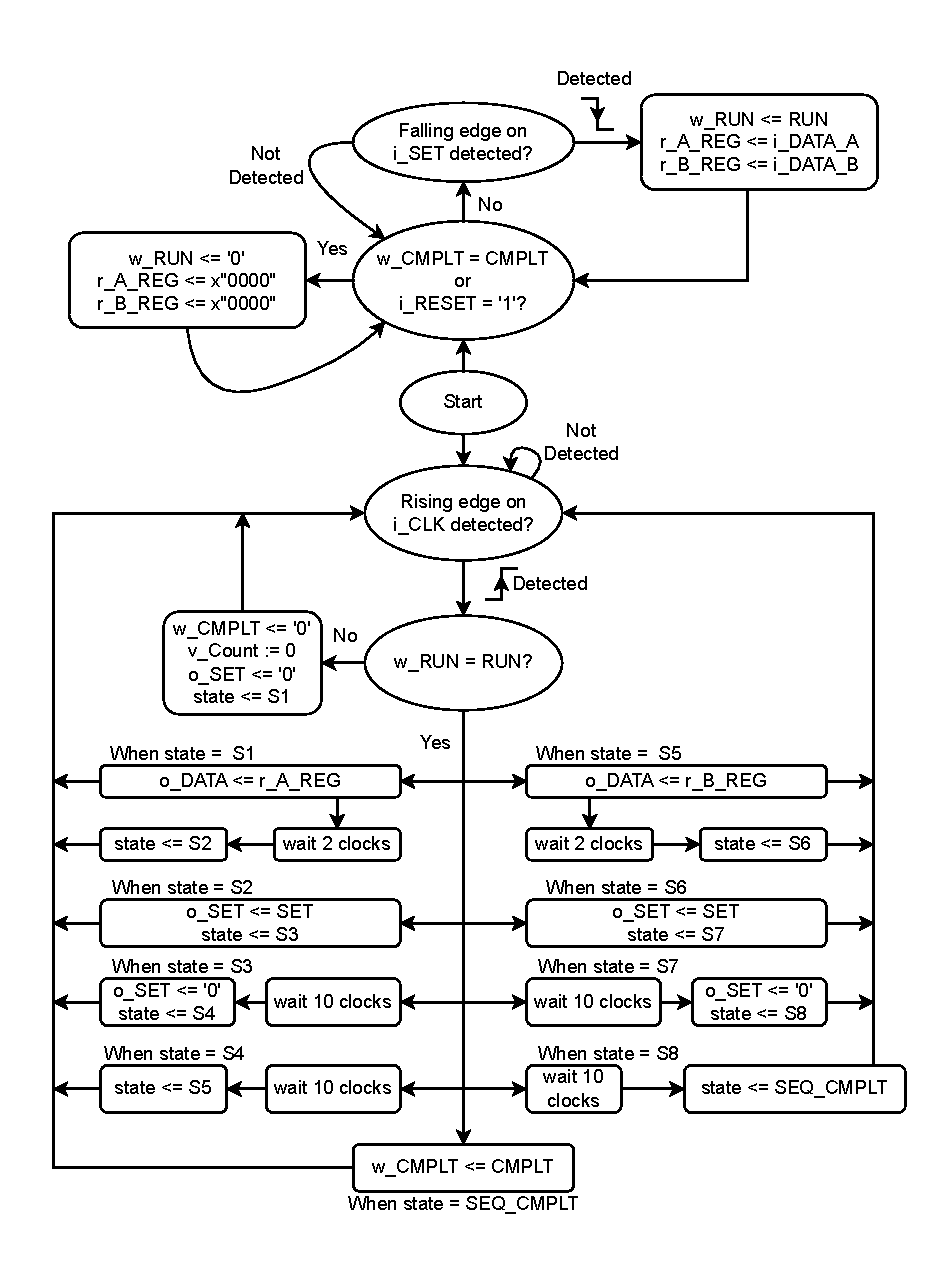
\includegraphics[clip, trim=0 0 0 0, width=1\textwidth]{Sections/7_SystemDesign/Figures/PSC_FSM20.pdf}
    \caption{The two FSMs inside the PSC block. The small FSM initiates the large FSM, that in turn hanldes the parallel to series conversion of the input current and voltage samples from the two ADCs.}
    \label{fig_7_2_11_PSC_FSM}
\end{figure}
The wait for clocks is a simple counter, an example can be seen in listing \ref{lst:7_2_11_PSC_COUNTER}. Here it can be seen that in state S4, the FSM will not advance to state S5 before 10 clocks have occurred, each clock takes \SIQ{5}{\nano\second} with a \SIQ{200}{\mega\hertz} master clock, resulting in a delay of \SIQ{50}{\nano\second}.

\lstinputlisting[language=c ,style = c,firstnumber=1, linerange=94-101, caption={Example of the counter to wait for x clocks used in the PSC FSM.}, label={lst:7_2_11_PSC_COUNTER}]{Sections/7_SystemDesign/Code/PSC.vhd}

The two FSMs shown in figure \ref{fig_7_2_11_PSC_FSM} shows that when a falling edge on "i\_SET" occures, indicating that the ADC data is ready, the large FSM will start running. Here the output to the IV Saver module is set to the data from ADC A (current), it then waits \SIQ{10}{\nano\second} to allow the output to settle. Hereafter is sets "o\_SET" high, this tells the next module in line that the output data is ready. It then waits \SIQ{50}{\nano\second} and sets "o\_SET" low, and waits another \SIQ{50}{\nano\second}. This process is then repeated for ADC B data (voltage).

Simulations show that this entire process takes \SIQ{265}{\nano\second}, it also shows that the time from ADC data A is set to ADC data B is set is \SIQ{130}{\nano\second}, well above the required \SIQ{100}{\nano\second}. This allows for a more realistically approximated data rate of $\frac{\SIQ{32}{\bit}}{\SIQ{265}{\nano\second}} = \SIQ{120}{\mega\bit/\second}$. This is more than required for a sample rate of \SIQ{1}{Msps}, and optimistically allows for a sample rate of \SIQ{3.75}{Msps}.

This could potentially be increased by reducing the delays in the FSM. The entirety of the VHDL code for the PSC module can be seen in appendix \ref{App:PSC_CODE}.